\chapter{Sistema Proposto}
\label{cap:Estrutura}

Para conceber a arquitectura do sistema de Monitorização de Rede orientado ao Processo (MRoP), foi necessário conhecer como os processos em nível utilizador comunicam com o exterior.
Após conhecer a arquitectura de rede do \textit{Linux}, foi imprescindível compreender a forma, como se processa a comunicação e a monitorização de rede.

Neste capítulo irá ser apresentada a constituição do sistema de rede do \textit{Linux}, desde o momento do envio dos dados pelo processo até que estes chegam à interface de rede e vice-versa.
Como esta visão é muito abrangente, apenas serão focados os pontos essenciais da arquitectura. 

---- TODO Dar a ideia de alguns pontos ----

Após esta visão geral do sistema de rede do \textit{Linux}, será apresentada a arquitectura proposta para o sistema de Monitorização de Rede orientado ao Processo (MRoP).



\section{Arquitectura de rede em \textit{Linux}}
\label{sub:network}

Os processos são instâncias de programas e estes num sistema multiprogramado partilham recursos.
Os processos necessitam de comunicar para obter dados, de forma a completar as suas execuções.
Estas comunicações podem ser efectuadas interna ou externamente ao sistema.
Em geral as comunicações externas processam-se através de uma interface de rede, para o que é necessário criar canais de comunicação.
A(s) interface(s) de rede são recursos do sistema, e por isso partilhadas pelos diversos processos.
Esta partilha é efectuada pelo núcleo, pois apenas este é capaz de a efectuar correctamente.

A criação de canais de comunicação é executada através da chamada ao sistema \textit{socket}.

----------- --------- ----------- qualquer coisa sobre a Norma posix ------------

\begin{figure}[htbp]
\centering
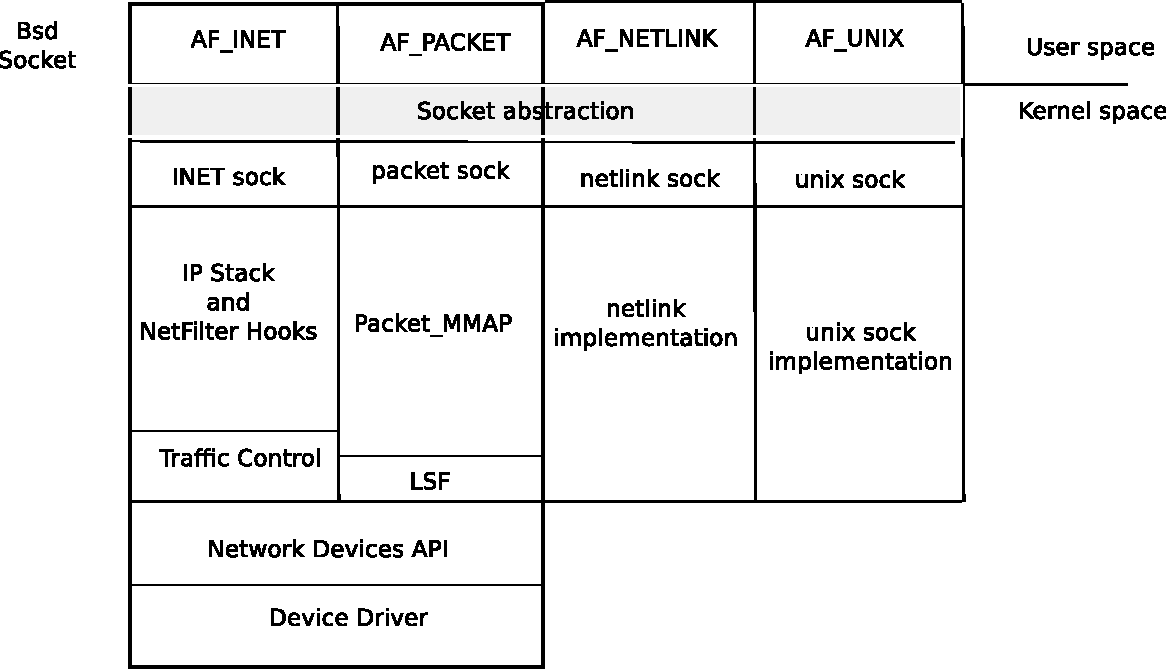
\includegraphics[scale=0.5]{network_arch.pdf} 
\caption{Arquitectura parcial de sockets do Linux}
\label{fig:network_arch}
\end{figure}

A chamada ao sistema \textit{socket} é efectuada para a criação de um canal de comunicação e este varia em função dos parâmetros familia, tipo e protocolo.

Existe um agrupamento em familia de endereços (\textit{Address Family}), que se destinam à comunicação remota ou local.
As comunicações locais podem efectuar-se entre processos (\textit{AF\_UNIX}), ou entre estes e o núcleo (\textit{AF\_NETLINK}), enquanto as remotas podem ter lugar sobre a \textit{internet}, dispondo igualmente de uma familia própria a \textit{AF\_INET}.

Os canais possuem um conjunto de funções (\textit{API}) bem definidas, para utilização e controlo, permintindo criar uma forma estruturada de comunicação.

Os administradores de sistemas necessitam filtrar o fluxo de informação que circula nas suas redes, pelo que se tem assitido ao desenvolvimento de sistemas de filtragem de comunicações, conhecidas por \textit{firewalls}.
Sendo o \textit{Linux} um sistema de operação frequentemente em ambientes de servidores, necessitou naturalmente deste controlo, daí que tenha sido desenvolvido o \textit{NetFilter}, uma \textit{firewall} que \color{red}filtra \color{black}o fluxo de dados que circulam na rede, entre o sistema e a periferia.

Para além da filtragem do fluxo de dados, existe um sistema de controlo do escalonamento do fluxo de tráfego, (\textit{Traffic Control}), que como o \textit{netfilter} é definido no núcleo, e permite ao administrador indicar quais os fluxos de dados prioritários ou que necessitam de determinada largura de banda, possibilitando-lhe efectuar para estes uma reserva antecipada.
 
Nas subsecções seguintes apresentar-se-ão diferentes constituintes da estrutura de rede do \textit{Linux}, começando pelo processo em nível utilizador até aos controladores de interfaces de rede.

\color{red}As últimas duas subsecções apresentarão a visão geral do fluxo de um canal de comunicação, envio e recepção, respectivamente.\color{black}

%Os processos em um sistema são instâncias de um programa, que partilha recursos físicos e lógicos da máquina.
%Os processos para aceder a alguns recursos, podem necessitar de efectuar comunicações com instâncias de outros programas, estes podem estar localizados na mesma máquina (processos locais), ou estar em outra máquina (processos remotos).

%Um processo para comunicar com outro através, utilizará as funcionalidades de rede do seu sistema de operação.
%Pois apenas este sabe gerir correctamente os recursos de rede.

 %Para isto um processo tem de efectuar o inicio da comunicação enviando alguns pacotes de inicio de sessão (caso o protocolo de comunicação necessite).
% Um processo em \textit{Linux} é uma instância de um programa que partilha recursos da máquina, físicos ou lógicos.
%\todo{muito pormenor}
% Os processos dentro do núcleo são instâncias de uma estrutura \textit{task\_struct} que contém diversos elementos pertencentes ao processo, tais como identificadores de processo, tabela de ficheiros abertos, zonas de memória atribuidas, permissões, etc.
 
% Um processo para utilizar as funcionalidades de rede necessita criar uma instância de um \textit{socket}, que fica referênciado através de um descritor de ficheiros (descritor de \textit{socket}).
% Tal como os ficheiros são acedidos em nível utilizador através de descritores os \textit{sockets} também são acedidos e manipulados através destes, apenas com chamadas ao sistema próprias para controlo e comunicação nestes canais.
 %Os \textit{sockets} são mapeados no sistema de ficheiros virtual, permitindo desta forma neste caso sobre a forma de \textit{sockets}, forma de comunicação sobre a rede.
% Estes descritores permitem ao processo identificar o \textit{socket}, para efectuar as comunicações.
 %Estas comunicações, bem como o estabelecimento destes canais de comunicação, são efectuadas através de chamadas ao sistema de operação.

%Falar aqui sobre qq coisa da estrutura de rede ... 
%Talvez tb imagem com um pouco da arquitectura ... básica 

%Falta falar sobre o netfilter ... sobre tc trafic control

%  Descrever um pouco esta parte ...
% Os canais de comunicação de rede estão organizados em familias de endereços, sendo a familia de endereços \textit{AF\_INET} utilizada para efectuar comunicações sobre a internet.
%Outras familias de \textit{sockets} existentes são \textit{AF\_NETLINK}, \textit{AF\_UNIX}, etc.
%A chamada ao sistema \textit{socket} é composta pela familia de endereços, pelo tipo e pelo protocolo.
%Desta forma generica é possível mapear diferentes tipos de comunicação, tais como \textit{INET} , \textit{NETLINK}, \textit{UNIX LOCAL}, em uma estrutura, o \textit{BSD socket}.

% A generalidade das aplicações utilizam os \textit{sockets} da familia \textit{AF\_INET}, para efectuar as suas comunicações sobre redes, sendo os principais tipos utilizados o \textit{INET\_STREAM} e \textit{INET\_DGRAM}.
% Estes dois tipos oferecencem canais orientados à conexão com estado e sem estado, respectivamente.


%Quando a chamada ao sistema \textit{socket} é efectuada, é criado uma nova instância de um socket e inicializados os respectivos campos com a informação dependente para a familia e tipo. 

%As principais chamadas ao sistema para estabelecer, terminar e comunicar sobre \textit{sockets} são: \textit{socket}, \textit{close}, \textit{connect}, \textit{bind}, \textit{listen}, \textit{accept}, \textit{send}, \textit{recv}, \textit{sendto} e \textit{recvfrom}. 


%Os file descriptors (socket descriptors) são os identificadores para os sockets. Os sockets são mapeados em ficheiros e estes em descritores de ficheiros. 

\subsection{Estrutura de um processo}
% ou recursos de rede de um processo

Um processo é a instânciação de um programa, sendo igualmente uma unidade de escalonamento de execução (\textit{task}) no sistema.
Este consome recursos (físicos e lógicos), partilhados com outros processos num sistema multiprogramado.
O núcleo para cada processo gere uma estrutura, \textit{struct\_task}, onde estão identificados todos os recursos a este atribuídos.
Esta estrutura contém apontadores para diversos recursos nomeadamente: zonas de memória requisitadas, canais abertos (ficheiros, \textit{sockets}, entre outros), contabilização de utilização de \textit{cpu}, apontadores para a sua árvore genealógica (pai, irmãos e filhos), etc.

A árvore genealógica anteriormente indicada contém o apontador para o pai (o processo que efectuou um \textit{fork}, para lhe dar origem), a lista de irmãos e de descententes.
O pai tal como cada um dos elementos da lista são também estruturas do tipo \textit{task\_struct}, pelo que é possível navegar pela árvore genealógica do processo.

Um dos recursos partilhados pelos diferentes processos é o acesso à rede, o que permite a comunicação com o exterior.
Para que as comunicações tenham lugar é necessário a alocação de canais de comunicação, cuja criação, utilização e destruição é efectuada pela \textit{API} definida no sistema de operação.
Quando um processo cria um canal, o núcleo devolve-lhe um identificador, que permite ao processo referenciar o canal dentro do núcleo, para controlá-lo e efectuar futuras comunicações.
No núcleo, este identificador é gerido na estrutura que identifica os canais abertos, pelo processo.

%A estrutura de canais abertos, permite abstrair qual o tipo de canal aberto, se foi um ficheiro, um socket, um \textit{pipe}, etc.

Para reconhecer qual o tipo do canal aberto, existem algumas funções específicas que o analisam e lhe permitem efectuar operações.
Assim, ao manipular um ficheiro existe a possibilidade de avançar e recuar, tendo como referência um determinado ponto.
Todavia, esta situação deixa de fazer sentido, quando se pretende controlar um \textit{socket} ou um \textit{pipe}, porquanto as comunicações nestes são destruídas quando consumidas, o que não acontece no ficheiro.
 

%Um processo para executar tem de ser carregado para memória e posteriormente ser agendado para execução através do escalonador de processos do núcleo.
% Um processo para o núcleo é uma estrutura com a informação sobre as zonas de memória, descritores de ficheiros abertos, informações sobre os tempos de execução, informações sobre a hierarquia de processos pertencentes a este, etc.
% Nos descritores de ficheiros abertos são também incluidos os descritores de \textit{sockets} abertos para comunicação. 

% Dentro do núcleo do linux a estrutura que tém a informação sobre um processo (\textit{task}), é a \textit{struct task\_struct}. 
% Nesta estrutura existe a informação sobre quais os ficheiros que a aplicação abriu.
% Como os \textit{sockets} são mapeados sob a forma de ficheiros, estes também se encontram nesta estrutura.


\subsection{Sockets e as suas famílias}
\label{sub:sockets}



Como o anteriormente referido em \ref{sub:network}, um processo para comunicar via rede, tem que criar um canal.
Estes são criados para efectuar comunicações locais ou remotas, e apesar das acções que podem ser efectudas serem comuns, o meio de transmissão é diferente, como diferentes são os canais e as formas utilizadas.
Os \textit{sockets} podem ser agrupados por familias de endereços \textit{Address Family}, que permitem especificar a forma de comunicação (local ou remota) utilizada.
Para caracterizar o canal não é apenas suficiente a especificação da familia, é igualmente necessário especificar o tipo de canal e o protocolo a utilizar, pois diferentes combinações de valores para estes parâmetros, traduzem-se em canais com diferentes funcionalidades.

\paragraph*{}
Nas subsecções seguintes irão ser apresentadas diferentes familias de endereços implementadas no núcleo, com especial ênfase para as familias \textit{UNIX}, \textit{INET}, \textit{NETLINK} e \textit{PACKET}.


%Como já foi indicado em \ref{sub:network}, um processo para comunicar tem de utlizar um \textit{socket}.
% Os \textit{sockets} para se diferenciarem devido às suas diferentes utilidades são definidos em  familias de endereços.
% Os \textit{sockets} para comunicação de internet utilizam o domínio \textit{AF\_INET}, que permite utilizar diferentes tipos de protocolos, tais como \textit{UDP} e \textit{TCP}.
% Estes protocolos são utilizados pela generalidade das aplicações quando necessita de comunicar com outro processo que utilize os mesmos protocolos de comunicação.


%Address Family para o INET, internet sockets para ipv4 e AF\_INET6 para ipv6

\subsubsection{AF\_UNIX}

Esta familia de \textit{sockets} é utilizada para efectuar a comunicação entre processos dentro da mesma máquina.
É um dos sistemas de \textit{Inter Process Communication (IPC)}, utilizado em sistemas Unix.
\color{red}Permite utilizar um ficheiro no sistema de ficheiros, como um canal de comunicações.\color{black}

\subsubsection{AF\_NETLINK}

A familia \textit{NETLINK} é utilizada pelos processos em nível utilizador para comunicar com o núcleo.
É possível efectuar comunicações ponto-a-ponto, ou multi-ponto, ou seja, é possível que um ou mais processos comuniquem com o núcleo, designadamente o \textit{netfilter}, o sistema de encaminhamento de pacotes de rede, o sistema de configuração de interfaces de rede, etc, através de um \textit{socket} nele criado.
Cabe aos processos em nível utilizador conectarem-se ao \textit{socket} definido no núcleo, que não é completamente passivo, podendo este iniciar comunicações assincronas com os processos.

Apesar das interfaces de rede serem configuradas através do programa \textit{ifconfig} em nível utilizador, que utiliza \textit{ioctl's} para as efectuar, outra ferramenta foi desenvolvida o \textit{ethtool} que através de \textit{socket netlink} permite efectuar estas configurações, uma vez que as \textit{ioctls} não permitem especificar correctamente os parâmetros ao contrário dos \textit{socket netlink}.


\subsubsection{AF\_INET}
\label{subsub:af_inet}

\textit{AF\_INET} é a familia de endereços utilizada na comunicação através da \textit{internet}, e que faz uso do protocolo \textit{IP versão 4} (ver figura \ref{fig:stack_tcp_ip}).

\begin{figure}[ht]
\centering
%url = http://upload.wikimedia.org/wikipedia/commons/3/3b/UDP_encapsulation.svg
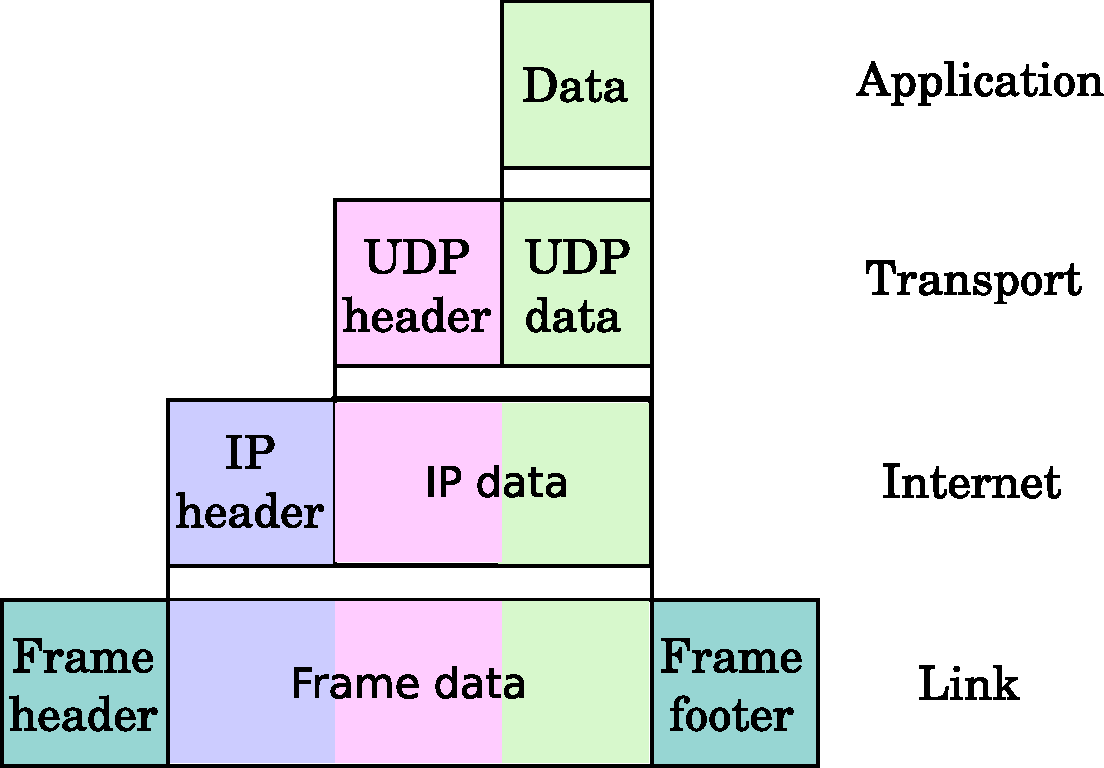
\includegraphics[scale=0.7]{UDP_encapsulation.pdf}
\caption{FIGURA APENAS PARA UDP NAO ESTA CORRECTA ......... Estruturação em camadas baseados em TCP/IP, obtido do sítio da internet http://upload.wikimedia.org/wikipedia/commons/3/3b/UDP\_encapsulation.svg}
\label{fig:stack_tcp_ip}
\end{figure}


A estruturação por camadas permite que a implementação de protocolos seja efectuada de forma simples e rápida, e ao utilizar as camadas inferiores como suporte para as superiores, aumenta a abstracção e complexidade dos protocolos.
Existem vários protocolos de nível transporte sobre \textit{IPv4}, sendo os mais utilizados o \textit{TCP} e \textit{UDP}, como o evidenciado pela figura \ref{fig:stack_tcp_ip}.
A criação de canais sobre o nível de transporte é efectuado utilizando a chamada ao sistema \textit{socket}, indicando para o parâmetro tipo os valores \textit{SOCK\_STREAM} ou \textit{SOCK\_DGRAM} para os protocolos \textit{TCP} e \textit{UDP} respectivamente.

O \textit{TCP} é utilizado para comunicações com controlo de fluxo de dados, que se adaptam ao canal existente tolerando a perda momentânea de pacotes, procedendo à sua retransmissão logo que possível.
O controlo das retransmissões é efectuado através do envio de pacotes (\textit{acknowledges}), que informam o transmissor dos que foram correctamente recebidos, permitindo-lhe reenviar os pacotes em falta.

O \textit{UDP} é um protocolo mais leve que o \textit{TCP}, pois não utiliza o controlo atrás referido, sendo habitualmente utilizado quando se está peramte a possibilidade de perda de pacotes durante a transmissão ou quando o controlo da retransmissão de pacotes é efectuado em camadas superiores.

Para além destes protocolos, existe ainda o \textit{SOCK\_RAW}, que permite acesso directo ao nível rede.
Este protocolo possibilita a criação de um canal que comunica directamente com o nível rede da pilha de protocolos \textit{TCP/IP}, permitindo executar protocolos de comunicação em nível utilizador.
Para utilizar \textit{sockets} através do modo \textit{RAW}, é necessário ter permissões de \textit{super user}, uma vez que é permitido o utilizador específicar parte dos cabeçalhos dos pacotes a enviar, sem que o núcleo os valide.
A não validação, pode proporcionar que pacotes maliciosos, isto é, com falhas deliberadas, possam ser introduzidos na rede.
 


\subsubsection{AF\_PACKET}
\label{subsub:af_packet}

A familia \textit{AF\_PACKET} comunica directamente com o controlador da interface de rede, possibilitando assim efectuar a monitorização de rede.
A utilização destes \textit{sockets} requer uma autorização de \textit{CAP\_NET\_RAW}, apenas disponível ao \textit{super user}.
Esta verificação previne que utilizadores não autorizados possam monitorizar, ou injectar pacotes na rede, influenciando o seu comportamento.
Dado que dispõe da possibilidade de enviar pacotes directamente para o controlador de rede, uma das suas utilizações é a implementação de protocolos de rede em nível utilizador.
Os de canais da familia \textit{AF\_PACKET} são frequentemente utilizado em sistemas de detecção de intrusos, pois permitem analisar os pacotes e detectar falhas na sua formatação.

TODO ------

Como a obtenção dos pacotes por estes canais, é efectuada antes da recepção destes pelos processos, existe a possibilidade de o \textit{NetFilter} bloquear a recepção de alguns pacotes, impedindo as aplicações de os receberem, não obstante este canal já os ter obtido para análise.

-----------


%Esta situação é devida ao posicionamento do \textit{NetFilter} em relação à monitorização de rede.
%No entanto ficaram visíveis à monitorização pois esta é efectuada antes de chegar aos \textit{Hooks} do \textit{netfilter}.
 
%Podem ser utilizados dois tipos \textit{SOCK\_DGRAM} ou \textit{SOCK\_RAW}.
 
%A utilização destes \textit{sockets} permitem a implementação de protocolos de rede, sem recorrer à \textit{stack} de protocolos IP dentro do núcleo.
% Para além desta funcionalidade esta é a forma de capturar os pacotes que circulam na interface de rede, permitindo assim efectuar uma análise do tráfego.

Como todos os pacotes recebidos pela(s) interface(s) de rede são obtidos por este canal, é necessário efectuar uma cópia destes e fornece-los à aplicação em nível utilizador.
Esta monitorização implica um peso extra na computação, por isso diversas técnicas, designadamente \textit{lazy cloning}, \textit{mmap}, etc, têm sido desenvolvidas no sentido de minimizá-lo.
A utilização de \textit{lazy cloning}, destina-se a apenas efectuar a cópia caso seja absolutamente necessária, permite reduzir a perda de eficiência do sistema, quando está a monitorizar os pacotes de rede.

-------------------------

TODO
A cópia do pacote é efectuada caso a avaliação do filtro indique que este deve ser copiado, caso contrário é terminada a execução em relação a esse pacote.

----------------------------------

% Por isso primeiro são avaliados para o processo de captura, caso sejam para captura a função \textit{blah blah} efectua a cópia da estrutura sk\_buffer e serão então adicionados ao \textit{ring buffer}.
% Se no \textit{ring buffer} não existir espaço para o número de bytes que devem ser capturados, é então descartado a cópia (libertado o espaço) e incrementado o valor de pacotes descartados pelo núcleo de sistema.


\subsection{NetFilter}


Este sistema, está implementado no núcleo do sistema de operação do \textit{Linux}, e controla o fluxo de dados dos processos para as interfaces de rede, bem como o oposto.
O \textit{NetFilter} está presente na \textit{stack TCP/IP} em apenas cinco pontos (\textit{PRE ROUTING}, \textit{LOCAL IN}, \textit{FORWARD} \textit{LOCAL OUT} e \textit{POST ROUTING}), em cada um dos quais existe uma lista de funções a ser executada sobre o pacote que foi recebido ou transmitido, sendo que após a finalização destas e dependendo do valor retornado, o pacote irá ou não prosseguir para as restantes camadas, até atingir o \textit{Traffic Control}(apresentado na subseccção \ref{sub:traffic_control} ou a aplicação, efectuando deste modo o controlo sobre o fluxo de rede.
O \textit{NetFilter} pode ser controlado pelo \textit{iptables}, uma ferramenta em nível utilizador, que através de regras, define o acesso dos dados das comunicações rede.
Estas são baseadas em endereços \textit{IP}, portos, interfaces de rede, etc, pelo que desta forma os administradores de rede não têm que conhecer internamente o \textit{netfilter}, apenas a arquitectura de rede, para definir as politicas de acesso do tráfego de rede ao sistema, permitindo ou bloqueando o tráfego com vista à satisfação dos objectivos pretendidos. 

Um dos componentes do \textit{netfilter} designado por \textit{connection tracking}, efectua o acompanhamento do inicio ao fim das ligações.
De forma a efectuar este acompanhamento necessita de conhecer os diferentes protocolos utilizados, para isso ele utiliza os \textit{connection tracking helpers}.
Estes ao conhecer o processo de estabelecimento de ligações/sessões indicam ao \textit{connection tracking}, se devem ser adicionados, removidos ou se a conexão passa a efectiva, ficando assim registada numa tabela de conexões estabelecidas até serem removidas.
De forma a não gastar todos os recursos de memória esta tabela tem dimensão fixa, e inicio de conexões que não ficam completas, ou por um temporizador que expirou ou por incorrecto estabelimento de sessão, são removidas permitindo que novas conexões possam ser adicionadas.
Tal como o \textit{netfilter} pode ser controlado por um programa em nível utilizador, esta componente \textit{connection tracking}, também pode ser controlada pelo administrador através do \textit{conntrack}.
Como se pode compreender este componente permite efectuar uma gestão mais eficiente e mais inteligente das conexões, sendo geralmente referido como \textit{firewall} como estado, é também utilizada para efectuar \textit{NAT} (\textit{Network Address Translation}) sobre as interfaces de rede, para permitir que máquinas no interior de uma rede possam aceder ao exterior utilizando a interface para o exterior, sem que tenham de ter endereços públicos, permitindo assim uma melhor gestão dos endereços públicos de \textit{IPv4}.

Como ao enviar dados o \textit{netfilter} termina no \textit{Traffic Control}, existe a possíbilidade de marcar pacotes com um identificador de forma a serem reconhecidos pelo \textit{traffic control}, de forma a ser efectuada uma gestão conjunta e inteligente do tráfego.

\subsection{Traffic Control}
\label{sub:traffic_control}
%------------------------------------------------------------------------------------------------------------
%TODO
% Dentro do núcleo do \textit{Linux} para além da \textit{firewall NetFilter} existe um mecanismo de controlo sobre os dados que circulam nas interfaces de rede.
% O principal propósito deste sistema é controlar a transmissão de dados, \textit{egress data transfer}.
% Quando os protocolos de nível 3 vão enviar os dados, para a camada de nível 2, estes são armazenados em \textit{QDisks} para posteriormente serem enviados.
% Com a necessidade de diferenciar os diferentes tipos de dados os administradores de sistemas podem diferenciar o trafego e armazená-lo em diferentes \textit{QDisks}, de forma a poder efectuar \textit{Quality of Service}.
%Apesar de ter estrutra para controlo dos dados que chegam da interface de rede o principal propósito é controlo do dados que saem através das interface de rede.

%------------------------------------------------------------------------------------------------------------

No núcleo para além do \textit{NetFilter}, que controla o fluxo de dados na rede, existe o \textit{Traffic Control} que efectua o escalonamento da transferências de dados para o exterior da rede.
O escalonamento do tráfego de rede é particularmente importante para os administradores desta, dado que a largura de banda é um recurso limitado, a sua gestão rigorosa é criteriosamente observada pelos administradores de rede.

A gestão é efectuada através de regras definidas em função da largura de banda, ritmo de envio, ou outros parâmetros.
O tráfego baseado nas regras atrás definidas, é agrupado em classes, que podem ter diferentes niveis de prioridade.
É ainda possível definir os algoritmos de escalonamento a utilizar, de modo a potenciar a eficiência da rede.

Quando está eminente o envio de um \color{red}segmento \color{black}\textit{IP} pela função \textit{ip\_output}, é transmitido para o \textit{Traffic Control}, onde o pacote é marcado com a \textit{tag} da respectiva classe, para posteriormente ser adicionado ao \textit{QDisk} correspondente.
O \textit{QDisk} é a estrutura de suporte à transmissão de dados efectuada pelo \textit{Traffic Control}, onde cada elemento desta estrutura é um \textit{sk\_buff}.


\subsection{Interfaces de rede}

A interface de rede é o dispositivo que efectua a transmissão e recepção de dados na rede.
Do ponto de vista do cpu, a interface de rede apenas efectua pedidos de interrupção, sendo que o restante trabalho é realizado pelo controlador de rede.
Este faz a ponte entre as funcionalidades de rede do núcleo e a interface de rede.

O núcleo mantém a informação sobre as interfaces de rede, inicializadas pelos seus controladores.
Esta, independentemente de estarem ou não em utilização, constam de uma lista duplamente ligada de \textit{net\_devices}.
Em cada posição desta lista existem informações referente a uma interface de rede, nomeadamente a informação sobre o seu endereço \textit{IP}, o seu endereço \textit{MAC}, etc, bem como outras configurações.

No registo de um novo controlador de interface de rede definem-se as operações a executar em determinados eventos, como a recepção e/ou transmissão de frames, a remoção da interface, etc.
Estas operações são definidas através de uma interface comum, a \textit{struct netdev\_ops}, que permite afectar a esta estrutura funções presentes nos módulos dos controladores, de modo a serem efectuadas as acções necessárias à utilização da interface de rede.

-------------------------

TODO
Falar sobre os controladores das interfaces de rede, que definem um conjunto de funções para serem desencadeadas em determinados pontos do envio ou recepcao de frames ... ndo (netdevice operations) 
 
-----------------------------------------

\subsubsection{Estrutura de um sk\_buff}
\label{subsub:sk_buff}

Os dados envolvidos no fluxo de comunicação e utilizados pelos controladores são os \textit{socket buffers}, estruturas do tipo \textit{sk\_buff}.
Esta estrutura contém diversos elementos, merecendo relevo os apontadores para a estrutura de rede do controlador, apontadores para secções do pacote (os diversos cabeçalhos pertencentes ao nível de rede e transporte), bem como o tamanho dos espaços alocados para estes e outros apontadores.

%Existem 4 apontadores para endereços de memória dentro da estrutura que definem os endereços de inicio e fim do pacote, bem como dos cabeçalhos.

%Falta boneco com esta informação ... fica mais realista.

\subsection{Recepção de dados}

%---------------------------------------OLD-----------------------------------------------------------

%A chegada de um pacote de dados à interface de rede desencadeia uma acção de interrupção da actividade do processador, permitindo quer este seja transferido para o sistema o mais cedo possível.
%Esta interrupção é efectuada através de um \textit{irq} pré-definido entre o controlador e a interface de rede. As interrupções são atendidas no processador desligando a atenção a todas as outras interrupções provenientes de outros dispositivos. %esta frase está ruim ...
%O processador deve estar o menor intervalo de tempo possível com as interrupções desligadas, antes de retornar da interrupção o sistema agenda a execução de uma função que irá terminar a recepção do pacote para a camada correcta da \textit{stack TCP/IP}.%ainda falta falar sobre DMA, interrupt mode too exclusive deve ser breve, encaminhar pelo processamento da stack tcp/ip 

%No processo de recepção da \textit{frame} é verificado se existem \textit{sniffers} registados, caso existam é passada uma referência sobre a frame, de forma a efectuar apenas a cópia da frame quando necessária.
%Esta situação é devida à possível existência de um filtro sobre a \textit{frame}, em que se não for necessário capturá-la, a cópia dos dados seja desnecessária, permitindo efectuar trabalho útil.

%Faltar falar que a frame segue para a stack tcp ip de forma normal ...

%Falta falar sobre o netfilter ... firewall do linux que existem 5 pontos de "entrada" onde existe algumas verificações .... 

%Faltar indicar que o processo está bloqueado à espera de input que lhe é copiado entre o nucleo e o processo em nivel utilizador por meio de o kiovec (talvez kernel io vector ...) 


%A variável global \textit{ptype\_base} do núcleo é uma tabela de dispersão aberta, que contém os tipos de controladores de protocolos de rede. Os diferentes protocolos endereçam uma função que recebe o pacote e sabe o que fazer com ele, passando pela \textit{firewall netfilter} terminando na cópia dos dados dos \textit{buffers} do núcleo para os do processo, que ficou bloqueado numa lista de espera através da chamada ao sistema de operação \textit{recv}, \textit{recvfrom} ou \textit{recvmsg}.

%----------------------------------------END OF OLD----------------------------------------------------

%O processo de recepção de pacotes pelas aplicações através de interfaces de rede, atravessa as diversas componentes apresentadas anteriormente em .... , ... e ... .

O sistema de monitorização de rede opera de forma opaca à normal utilização de rede, pelas aplicações, desta forma quando um pacote chega à interface de rede, esta envia um pedido de interrupção da computação ao cpu, para que este atenda o pedido da interface de rede.
Neste ponto é desligada a atenção do processador a novas interrupções, passando a computação para o controlador da interface de rede.
Uma vez que a atenção do processador a novas interrupções está desligada, a computação deve ser o mais breve possível a reiniciar-se a atenção do processador a novas interrupções e o normal funcionamento seja retomado.
Apenas a computação crítica é efectuada diferindo a restante execução, através da invocação de um \textit{softirq}, para que seja terminado o tratamento dos pacotes que chegaram à interface.
%O escalonamento do \textit{softirq} potencia o aproveitamento dos recursos ao equilibrar a execução de interrupções com as restantes tarefas.

Os pacotes recebidos são entregues aos \textit{sniffers} registados no sistema, antes de o serem aos \textit{packet handlers} respectivos.
A monitorização de rede é efectuada pelos \textit{sniffers}, sendo os pacotes entregues a cada um deles, para que possam proceder à sua análise.
Cada \textit{sniffer} tem um filtro associado escrito em linguagem \textit{bpf}, a ser executado na máquina virtual implementada para o efeito.

%\begin{lstlisting}
%struct sock_filter {    /* Filter block */
%	__u16	code;   /* Actual filter code */
%	__u8 	jt;     /* Jump true */
%	__u8 	jf;     /* Jump false */
%	__u32	k;      /* Generic multiuse field */
%};

%struct sock_filter filter = {
%	.code =  BPF_RET,
%	.k = 100
%};
%\end{lstlisting}

%Este filtro indicado pela variavel \textit{filter} (linha 8) descrito em linguagem \textit{bpf}, ao ser executada pela máquina virtual, indica que devem ser capturados os primeiros 100 bytes de cada pacote.

\subsection{Transmissão de dados}

Uma aplicação em nível utilizador transfere dados sobre a rede através de chamadas ao sistema de operação, sendo que estas podem ser \textit{send}, \textit{sendto}, \textit{sendmsg}.
Neste ponto de entrada os dados são copiados e sobre eles são efectuadas diversas verificações.

Seguidamente são utilizadas estruturas e funções do núcleo, fluindo pela \textit{stack TCP/IP} e \textit{netfilter} até ser entregue ao controlador da interface de rede.

Os dados gerados pelas diversas camadas da \textit{stack} são agregados numa estrutura \textit{sk\_buffer} para ser adicionados a uma fila para ser enviados pela ferramenta \textit{traffic control}.
Quando esta ferramenta irá enviar os dados para o controlador é passada a referência sobre este pacote para os \textit{sniffers} registados, sendo apenas efectuada uma cópia dos dados caso o pacote seja recolhido para maior análise. Os dados passados ao controlador da interface de rede são então transferidos para a interface de rede, e daí para o seu destino.

Quando a aplicação está a executar e efectua uma chamada ao sistema de operação, o sistema muda de modo e executa dentro do núcleo "em nome da aplicação".
 Durante parte da execução da chamada ao sistema de operação é possível referenciar qual o processo que efectuou a chamada, pois caso a chamada seja sincrona, é agendada um processamento sobre os dados e a aplicação fica bloqueada à espera de ser re-escalonada através da função \textit{schedule}.
 O sistema de ficheiros mantém a referência sobre quais os ficheiros/sockets abertos para cada processo e é possível obter qual o processo a que cada descritor de ficheiros pertence. % back pointers ... nos sockets ... binded de uma porta a um processo ... pode nao ser a chamada bind ... 

\section{Desenho e arquitectura do MRoP}
\label{sec:mrop_architecture}

O sistema proposto foi desenvolvido procurando cumprir os seguintes requisitos:
\begin{itemize}
\item seleccionar as comunicações envolvendo apenas um processo (ou um conjunto de processos);
\item manter a compatibilidade com o sistema já existente, incrementando a sua funcionalidade;
\item minimizar eventuais perdas de desempenho;
\item a implementação deve envolver poucas alterações ao código do sistema, para facilitar a sua manutenção e evolução com as novas versões do sistema \textit{Linux}.
\end{itemize}

Assim, o sistema criado está dividido em quatro componentes principais: filtragem dos pacotes de rede, instrumentação das chamadas ao sistema, repositório do estado das interacções via rede, e controlo e informação sobre o estado da monitorização (ver figura \ref{arquitectura}).
A função de filtragem, é invocada por um \textit{hook} que estende o \textit{LSF}, permite que apenas o tráfego do processo alvo seja analisado pelo restante sistema de fitragem do \textit{LSF}.
Relativamente à componente instrumentação das chamadas ao sistema (ou outras funções contidas no sistema de rede), actualiza a componente repositório de dados, onde é mantido o estado das interacções via rede do(s) processo(s) alvo, com as efectuadas pelo processo.
Existe ainda um sistema para controlo/configuração destinado a obter informação sobre o estado da monitorização.

\begin{figure}[htbp]
\begin{center}
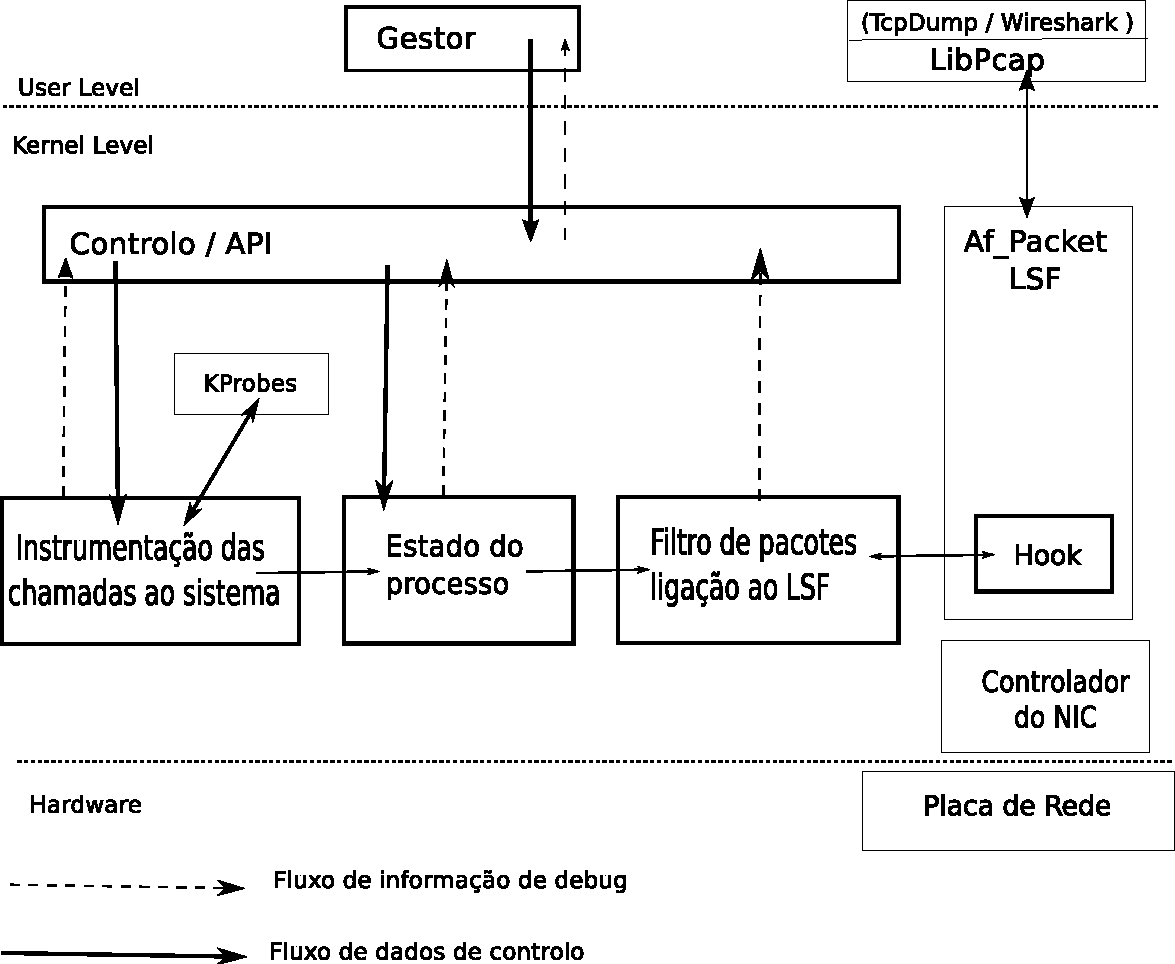
\includegraphics[scale=0.5]{arquitectura.pdf} 
\caption{Arquitectura da solução}
\label{arquitectura}
\end{center}
\end{figure}

Este sistema, MRoP, captura os pacotes de rede de um processo, sem que exista um conhecimento prévio sobre o(s) protocolo(s) ou portas utilizadas.
A utilização de um sistema de instrumentação do núcleo foi necessária apenas para monitorizar as chamadas envolvendo \emph{sockets}, e identificar o processo responsável, permitindo desta forma obter e manter permanentemente actualizada a informação sobre o estado do processo alvo.
De forma a minimizar a redução de desempenho, todo o sistema foi desenvolvido no núcleo do \textit{Linux}, sem alterações nas interfaces já existentes.
Assim, ferramentas que façam uso da biblioteca \textit{LibPcap}, como o programa \textit{tcpdump} ou as suas variantes, podem beneficiar desta extensão sem qualquer alteração e sem impacto relevante no seu desempenho.

%---------------------------------------------------------------------------------------------------------
%TODO
%A arquitectura foi pensada para ser executada de forma ortogonal ao sistema utilizado.
% Desta forma não existe a necessidade de recompilar programas antigos.
% Para além desta situação novas aplicações podem utilizar esta ferramenta de forma transparente.

%Esta ferramenta foi desenvolvida para os processadores x86 e x86\_64 pois nestas arquitecturas existe suporte para o sistema de monitorização KProbes \ref{}, sendo esta a unica dependência especifica que a ferramenta irá ter.

%As diferentes partes da ferramenta foram desenvolvidas de forma a poderem ser modificadas em separado permitindo um melhor aproveitamento da modularização.
Este módulo do núcleo foi desenvolvido em quatro componentes, que a seguir se apresentam:

%---------------------------------------------------------------------------------------------------------


\subsection{Instrumentação das chamadas ao sistema de rede}
\label{sub:mon_syscalls}

A principal relevância deste sistema, assenta na gartantia de que todas as interacções desencadeadas por um processo com o exterior sejam detectadas.
Para atingir esse objectivo, foi necessário recorrer à monitorização das chamadas ao sistema de rede ao nível do núcleo, possibilitando reduzir as cópias de dados e as trocas de contexto.
Fazendo uso do sistema de monitorização \textit{KProbes} foi possível realizar a monitorização sob o limitando conjunto de chamadas ao sistema, nomeadamente: \textit{sendto}, \textit{recvfrom}, \textit{bind}, \textit{accept}, \textit{connect} e \textit{close}.


%Na realidade constatou-se que chamada ao sistema close, ao ser utilizada intensivamente por todo o sistema de ficheiros, poderia degradar desnecessariamente o desempenho.
%Desta forma, decidiu-se aplicar a monitorização à função interna \texttt{sock\_close}, garantindo apenas a monitorização das chamadas close sobre os sockets, reduzindo significativamente o número de eventos face às chamadas ao sistema do \texttt{close}.

\subsection{Estado do processo}
\label{sub:data_repository}

O estado dos portos dos protocolos \textit{TCP} e \textit{UDP} em uso no processo alvo é mantido num repositório de dados e permanentemente actualizado pelo componente anteriormente referido em \ref{sub:mon_syscalls}.
A árvore \textit{Red and Black} já disponível no núcleo do sistema, foi a estrutura dados escolhida para produzir o repositório pretendido.

O conteúdo de cada folha da árvore é uma estrutura com duas listas de elementos, cada uma contendo endereços IP utilizados pela aplicação.
A chave de indexação das folhas é o número do porto, desta forma a árvore poderá conter no máximo 65535 elementos, por ser este o número máximo de portos em utilização por um endereço \textit{IP}.
No pior caso, a procura de um porto na árvore necessitará de efectuar dezasseis iterações, uma vez que \begin{math}\log _2 65536 = 16 \end{math}.

%\td{conteúdo? ip, interface, porto udp, porto tcp, etc??}
  O uso deste tipo de estrutura permite obter um bom compromisso entre o tempo de acesso à estrutura e a quantidade de memória utilizada.


\subsection{Filtro de pacotes}
\label{sub:packet_filter}

A função de filtragem implementada neste sistema assenta no estado do processo alvo, mantido pelos módulos anteriormente descritos.
Através da extensão do \textit{LSF} com um \textit{hook}, este quando ligado invoca esta filtragem que devolve ao \textit{LSF} informando-o se o pacote deve ou não ser capturado.
Se for capturado indica que este pacote pertence ao processo alvo, caso contrário irá avaliar as restantes regras de filtragem definidas.
Mantém-se assim a compatibilidade e os beneficios da utilização do \textit{Linux Socket Filter}.
Quando não existe uma ligação (\textit{hook}) activa, assiste-se a um ligeiro decréscimo no desempenho na utilização da filtragem estática.
Tal facto deve-se apenas à necessidade de constatar se a ligação está ou não activo.

Como se pode verificar este sistema interage com o filtro estático do \textit{LSF}, efectuando uma conjunção entre o filtro definido pelo utilizador e a captura do tráfego da aplicação a ser monitorizada.


\subsection{Controlo e Informação}
\label{sub:data_information}

Para facilmente controlar e configurar o sistema desenvolvido foi definida uma interface baseada em ficheiros virtuais numa directoria do (\textit{DebugFS}).
Estes ficheiros com permissões apenas acessíveis ao utilizador \textit{root}, impedem o acesso por parte dos restantes utilizadores da máquina ao sistema de monitorização.
%Os ficheiros de controlo definidos foram \textit{option}, \textit{pid}, \textit{ppid} e \textit{tgid}.


% O primeiro ficheiro permite controlar a análise e a informação da árvore.
% Dependendo do valor a escrever em \textit{option} o sistema poderá proceder a uma análise dos \textit{sockets} do processo (identificado em \textit{pid, ppid, tgid}), e carregar essa informação para a àrvore do estado do processo, bem como poderá remover todos os elementos da àrvore se for essa a opção escrita para o ficheiro.
% Como foi indicado os restantes ficheiros permitem definir o(s) processo(s) a monitorizar.
% Pode ser indicado um processo ou fluxos de execução pertencentes ao grupo do processo.
% Os ficheiros de informação \textit{filter\_stats}, \textit{syscalls\_calls\_stats} e \textit{tree\_info} foram definidos para obter estatísticas dos pacotes analisados e das entradas/retornos das funções instrumentadas, bem como dos elementos presentes na árvore (dados dos sockets activos do processo).

%\subsubsection{Mais info}
%a não utilização de ioctl para o debug ... 
%A estratégia foi separar os diferentes componentes e a criação de um módulo de \textit{debug} para que pudesse existir uma forma de acesso à monitorização por parte do nível de utilizador, sem que exista a necessidade de criar ou alterar chamadas ao sistema ou suas opções.



\section{Conclusão}

Algumas ideias para concluir este capitulo ...

